

\section{Fast Computations for Robust and Vanilla CP with Lipschitz bounds}
\label{sec:efficient_robust_sets}

In this section, we introduce Lipschitz bounds for neural networks and use their validity across the totality of the support of $\inputspace$ to enable fast computations of conservative and restrictive scores. 

\subsection{On the Lipschitz Constant of Neural Networks}
%
\begin{definition}[Lipschitz constant]
    A neural network classifier $f: \inputspace \rightarrow \Reals^{c}$ is said to be $L$-Lipschitz in $\ell_p$ norm if it verifies the following behavior:

    \begin{equation}
        \forall(x,y) \in \inputspace^2, \| f(x) - f(y) \|_p \leq L.\| x - y \|_p
    \end{equation}
\end{definition}

Importantly, most deep neural networks -excluding attention based architectures~\cite{havensfine}- are Lipschitz continuous.

\paragraph{Estimating Lipschitz constants of neural networks} Computing the exact Lipschitz constant of deep neural networks is an NP-hard problem as stated in \cite{lipschitznphard}. In order to mitigate this issue, some methods like \cite{wang2024on} compute over-estimations of the Lipschitz constant of the network, for instance by computing the product of the Lipschitz constant of the network's layers. Unfortunately, these methods currently offer very loose estimations, any breakthroughs in that field would benefit our framework.


A more popular alternative to ad-hoc computation lies in the field of ``Lipschitz by design'' architectures. This very active field relies on the seminal work of \cite{sortingout} to provide efficient weight re-parametrizations that ensure 1-Lipschitz behavior in $\ell_2$ norm (in general). Some notable examples include Riemannian optimization inspired implementations \cite{lezcano2019trivializations}, or even performance-focused implementations with reduced computational overheads during training \cite{sll,boissin2025adaptiveorthogonalconvolutionscheme}. Using Lipschitz-constrained networks introduces the several advantages. First and foremost, Lipschitz-constrained networks allow \textit{explicit} control of their placement on the robustness-accuracy trade-off \cite{payattentionlossunderstanding}. Also, additional orthogonality constraints on these networks have been shown to result in generally tighter Lipschitz bounds. Finally, these constraints also mitigate the gradient vanishing problem \cite{li2019preventing} and allow for more efficient training. 

Therefore, Lipschitz-constrained networks have two main advantages: their training objective explicitly promotes robustness and the estimation of the Lipschitz constant is locally tight. These particular traits will be key to getting fast and tight estimations of the conservative and restrictive scores.

\subsection{Computing Conservative and Restrictive Conformal Scores}

\begin{figure}[!t]
    \centering
    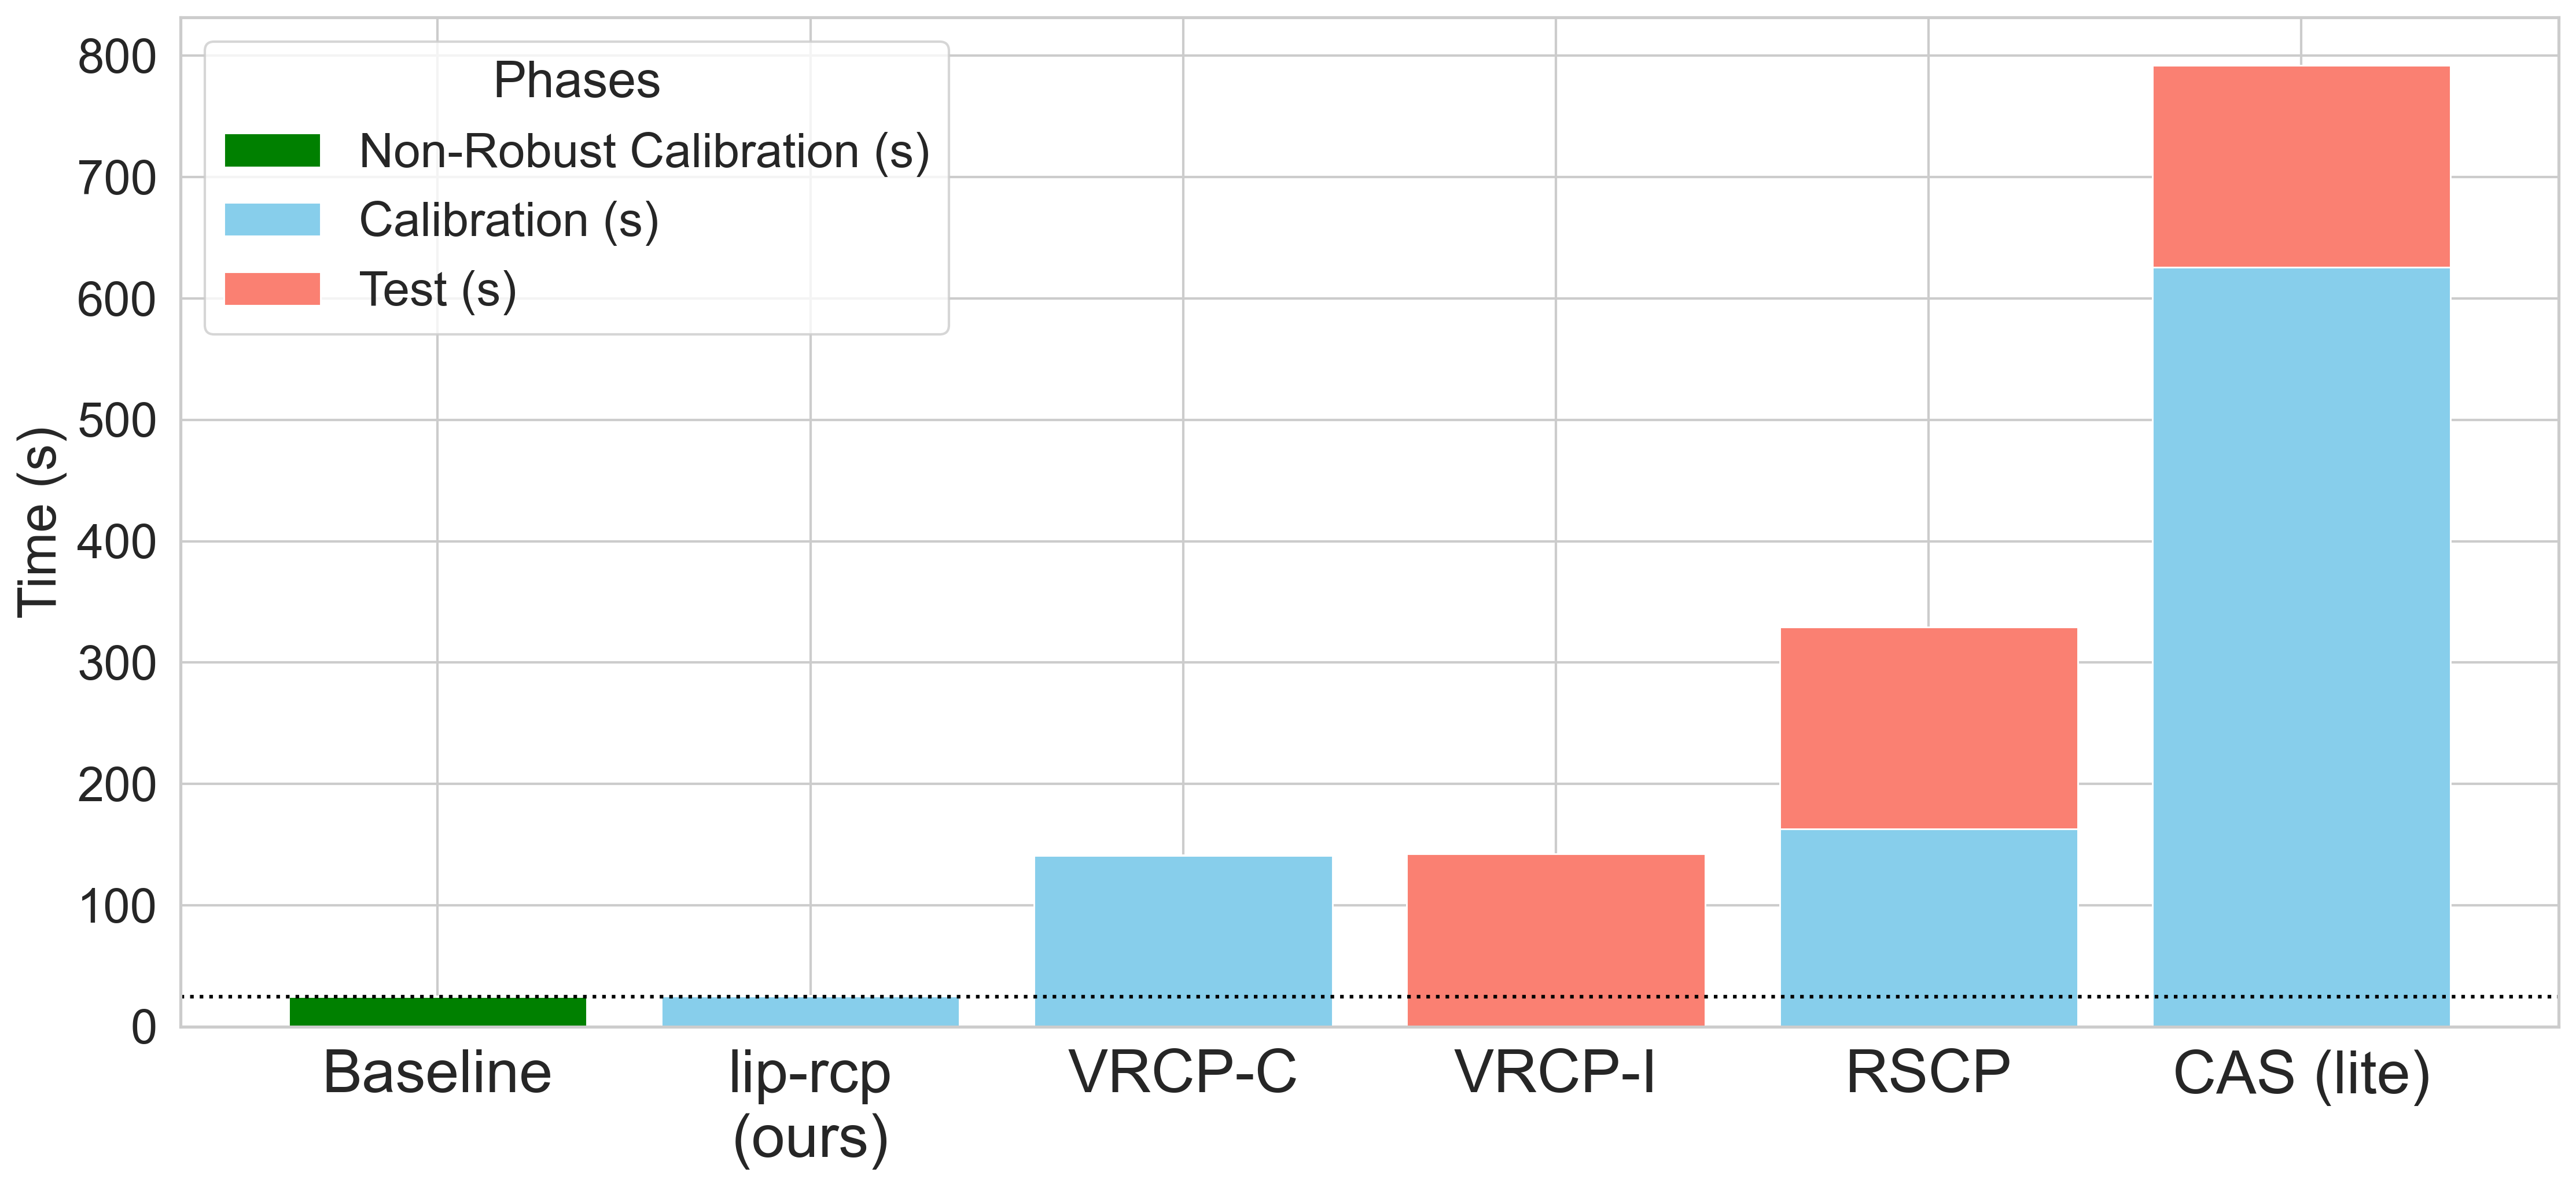
\includegraphics[width=0.8 \linewidth]{speed.png}
    \caption{
    Calibration and test time
    on the \textsl{CIFAR-10} dataset for different robust CP methods. Our method has negligible overhead compared to vanilla CP.  
    Here we use $n_\mathrm{cal} = 4750, \ n_\mathrm{test}=4750$ and $n_{\mathrm{mc}} = 1024$, \emph{CAS (lite)} corresponds to the version of \emph{CAS} that leverages CDF-Aware smoothed Prediction Sets only at calibration time. 
    }
    \label{fig:speeeed}
\end{figure}

\begin{figure*}[t!]
    \centering
    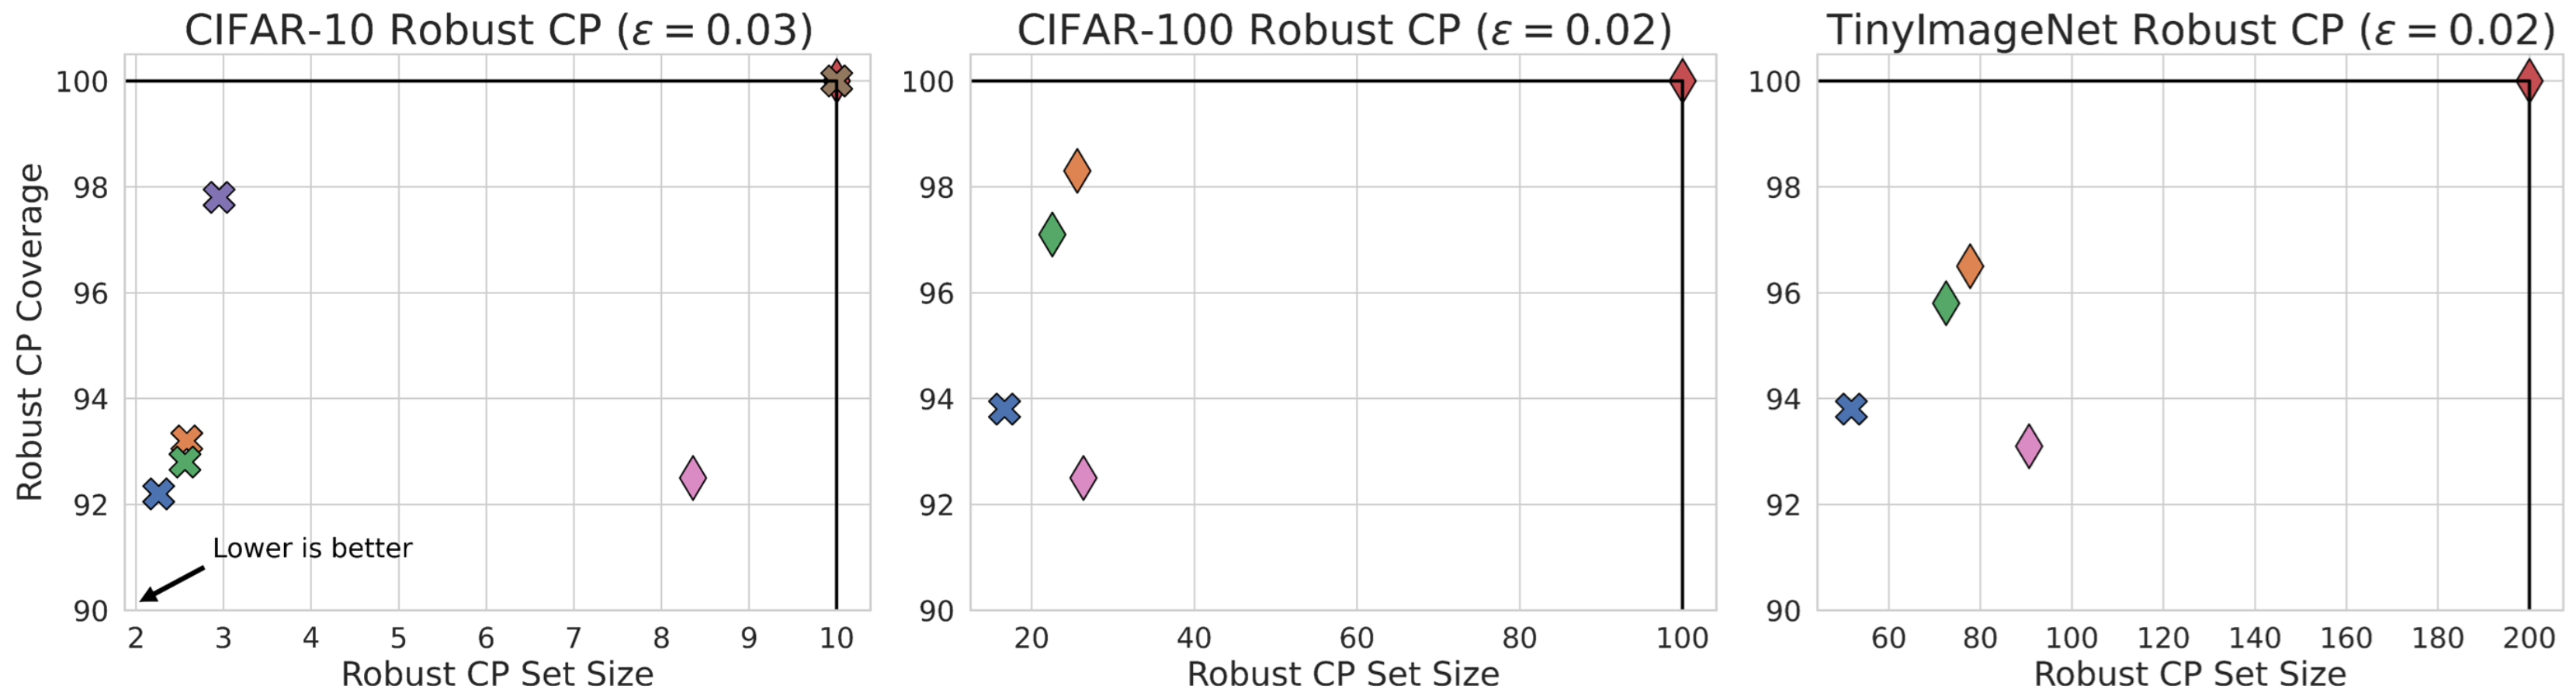
\includegraphics[width=1.0\linewidth]{banner_results.png}
    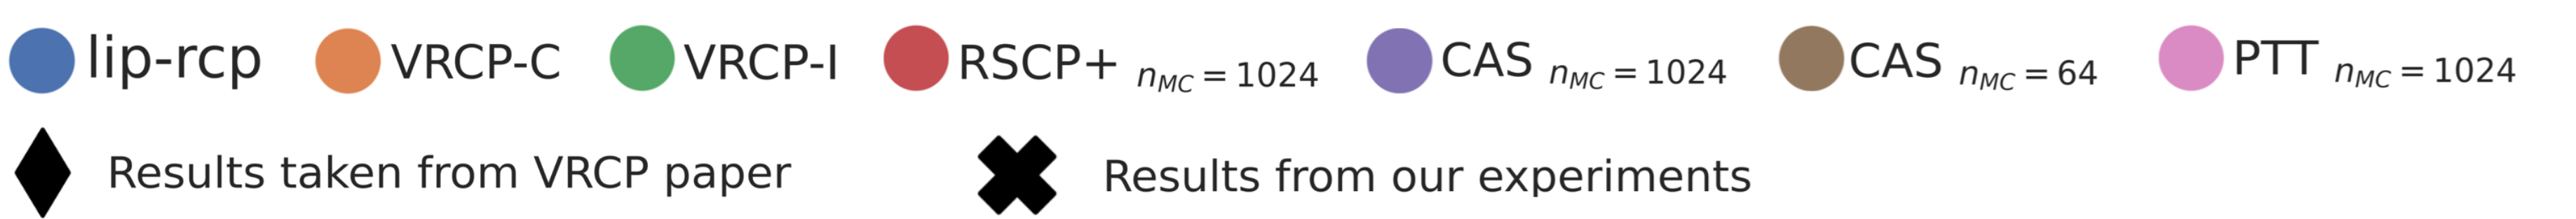
\includegraphics[width=0.65\linewidth]{banner_results_legend.png}
    \caption{
        Robust CP set sizes and empirical coverage values across different classification datasets for $\alpha=0.1$. Ideally, the best robust CP sets are small while nearly achieving the desired coverage guarantee (bottom left corner)}. We plot values that were taken from the \emph{VRCP} paper with diamonds while our measurements are plotted as crosses.
    \label{fig:fastcp_results}
\end{figure*}


In this section, we use the global Lipschitz bound of our networks to efficiently estimate the conservative and restrictive prediction sets at model inference. We call our method \emph{lip-rcp}. These estimations are then used to construct robust CP sets and audit the robustness of vanilla CP as per \S~\ref{sec:vanillacoverage}. 
Our approach can be connected to the Lipschitz properties exhibited by the smoothed classifier introduced in \emph{RSCP}. 

However, at inference time, most Lipschitz weight re-parametrization schemes can be exported as a set of regular neural network weights to eliminate any computational overhead compared to their unconstrained counterparts.


\paragraph{Lipschitz score bounds} Assuming the non-conformity score $s(x,y)$ can be expressed as $\psi(f(x),y)$ such that $f$ is an $L_n$-Lipschitz classifier and $\psi(\cdot,y)$ is $L_s$-Lipschitz in $\ell_p$ norm for all $y \in \labelspace$, we can write: 
\begin{equation}
    \forall y \in \labelspace, | s(x, y) - s(x+\delta,y) | \leq L_n \cdot L_s \cdot \| \delta \|_p. 
\end{equation}
%
This induces the following bounds $\forall \Tilde{x} \in \bouleps(x), \forall y \in \labelspace$ : 
%
\begin{equation}
    \underbrace{s(x,y) - L_n \! \cdot \! L_s \! \cdot \! \epsilon}_{=\underline{s}_\emph{lip-rcp}(x,y)} \leq s(\Tilde{x},y) \leq \underbrace{s(x,y) + L_n \! \cdot \! L_s \! \cdot \! \epsilon}_{=\overline{s}_\emph{lip-rcp}(x,y)}
\label{eq:lipschitz_ineq}
\end{equation}
%
\paragraph{Score function} 
In the literature of CP, the Least Ambiguous Classifier (LAC) score, usually based on the softmax function, is classically used to provide conformal scores. 
One alternative we propose is to use a \textit{sigmoid} based conformal prediction score that we call the LAC sigmoid score:

\begin{equation}
    s(x,y) = 1 - \text{sigmoid}\left(\frac{f(x)_y - b}{T}\right).
\label{eq:sig_score}
\end{equation}

Importantly, the Lipschitz constant of this score function is $L_s = 1 / (4 \times T)$ w.r.t $f(x)_y$. 

Note that this score differs from the \emph{PTT} score of \cite{rscp} given that the value of $f(x)_y$ is directly passed through the sigmoid of temperature $T$ and bias $b$. No ranking transformation requiring an extra data split is applied. Furthermore, replacing $s(x,y)$ with $1-\text{softmax}(f(x)/T)_y$ would be similar in spirit. However, some experiments suggest that it might lead to larger prediction sets; see Appendix~\ref{app:scores}.

\paragraph{Unified calibration and test-time process} The certificates provided by \emph{VRCP} hold locally around data points $(X_i,Y_i)_{\CalDataset}$, and \emph{VRCP} distinguishes two possible robust CP procedures: robust calibration (\emph{VRCP-C}) or robust inference (\emph{VRCP-I}). However, using global Lipschitz bounds eliminates that need. Indeed, a robust calibration threshold $q_{\alpha,\epsilon}$ defined on scores $\underline{s}_\emph{lip-rcp}(x,y)$ of Eq.~\eqref{eq:lipschitz_ineq} 
yields the same results as robust inference given that the quantile computation is translation equivariant.


\paragraph{Efficient computation} To estimate the conservative and restrictive scores of Def.~\ref{def:union-inter-metaset}, we can simply leverage the expression of the bounds of Eq.~\ref{eq:lipschitz_ineq}. We detail the time complexities for the computation of a non-conformity by different certifiably robust CP methods in Table~\ref{tab:time_complexities}. In addition, we provide runtimes for the calibration and testing steps of different methods in Fig.~\ref{fig:speeeed}.

\begin{table}[h]
  \centering
  \begin{tabular}{lcc}
    \toprule
    Method         & Cal. complexity & Test complexity \\
    \midrule
    RSCP           & \(\mathcal{O}(n_{\mathrm{mc}})\)              & \(\mathcal{O}(n_{\mathrm{mc}})\)               \\
    CAS            & \(\mathcal{O}(n_{\mathrm{mc}})\)              & \(\mathcal{O}(n_{\mathrm{mc}}\times t_b)\)     \\
    VRCP-I         & \(\mathbfcal{O}(1)\)                             & \(\mathcal{O}(t_v)\)                            \\
    VRCP-C         & \(\mathcal{O}(t_v)\)                           & \(\mathbfcal{O}(1)\)                             \\
    lip-rcp (ours) & \(\mathbfcal{O}(1)\)                             & \(\mathbfcal{O}(1)\)                             \\
    \bottomrule
  \end{tabular}
  \caption{Time complexity for computing a single non-conformity score. Here \(n_{\mathrm{mc}}\) is the number of Monte Carlo samples, \(t_b\) the CAS‐bound cost, and \(t_v\) the VRCP solver cost. \emph{lip-rcp} is the only method with constant‐time calibration and inference.}
  \label{tab:time_complexities}
\end{table}
